\documentclass[a4paper,12pt]{article}

\usepackage{array}
\usepackage[utf8x]{inputenc}
\usepackage[T2A]{fontenc}
% \usepackage[russian, english]{babel}
\usepackage[english,russian]{babel}

% Опционно, требует  apt-get install scalable-cyrfonts.*
% и удаления одной строчки в cyrtimes.sty
% Сточку не удалять!
% \usepackage{cyrtimes}

% Картнки и tikz
\usepackage{graphicx}


% Некоторая русификация.
\usepackage{misccorr}
\usepackage{indentfirst}
\renewcommand{\labelitemi}{\normalfont\bfseries{--}}
% Увы, костыль
% \addto\captionsrussian{\def\figurename{{\cyr\CYRR\cyri\cyrs\cyru\cyrn\cyro\cyrk}}}


% Увы, поля придётся уменьшить из-за листингов.
\topmargin -1cm
\oddsidemargin -0.5cm
\evensidemargin -0.5cm
\textwidth 17cm
\textheight 24cm

\sloppy

% Оглавление в PDF
\usepackage[
bookmarks=true,
colorlinks=true, linkcolor=black, anchorcolor=black, citecolor=black, menucolor=black,filecolor=black, urlcolor=black,
unicode=true
]{hyperref}



\title{ Методы вычислений \\Отчёт по лабораторной работе \textnumero 1 \\  }

\author{Кузьмин А.}
\date{20 мая 2013}

\begin{document}

%\maketitle

\begin{titlepage}
\newpage
\begin{center}
МГТУ им. Н.Э. Баумана \\		% \\ означает перенос
\hrulefill %горизонтальная черта
\end{center}

\vspace{10em}
\begin{center}
\Large Методы вычислений \\
\vspace{1em}
Отчет по лабораторной работе \textnumero 1  
\end{center}


\begin{center}
\textsc{\textbf{Распространение тепла в стержне}}
\end{center}

\vspace{15em}
\begin{flushright}
Кузьмин А. \\
Студент группы ИУ7-29 \\
Вариант 19
\end{flushright}
\vspace{\fill}
\begin{center}
Москва 2013
\end{center}
\end{titlepage}


\newpage

\section{Постановка задачи}
\subsection{Формулировка задачи}

Найти температуру $u(x,t)$ тонкого стержня длиной $l$ с теплоизолированной боковой поверхностью, на концах которого задан температурный режим. Коэффициент теплопроводности $K$ меняется в зависимости от температуры по заданному закону \( K=K(u) \). В начальный момент времени \( t=0 \) стержень находится при фиксированной температуре $u_0$ по всей длине. Найти момент времени $T$, в который температура в середине стержня будет максимальной.

\subsection{Исходные данные}
\newcolumntype{M}{>{\centering\arraybackslash}p{5cm}}
\newcolumntype{C}{>{\centering\arraybackslash}p{3cm}}
\newcolumntype{T}{>{\centering\arraybackslash}p{2cm}}

    \begin{tabular}{|C|M|}
        \hline
         \(l\) & 1 \\ \hline
         \(\rho\) & 1 \\ \hline
         \(c\) & 0.5 \\ \hline
         \(u_0\) & 0.1 \\ \hline
         \(a\) & 1 \\ \hline
         \(b\) & 2 \\ \hline
         \(\sigma\) & 0.25 \\ \hline
         \(t_0\) & 0.5 \\ \hline
         \(Q\) & 10 \\ \hline
    \end{tabular}

\subsection{Тепловой поток}
На правом конце стрежня тепловой поток равен 0.


На левом конце стрежня:
$$W_3(t)=\left\{\begin{array}{lll} 2Q(t_0-t),&0\le t < t_0; \\ 0,&t\ge t_0; \end{array}\right.$$

\subsection{Коэффициент теплопроводности}
 \(K(u) = a + bu^\sigma\)

\newpage
\section{Теоретические сведения}
\subsection{Краевая задача}

\begin{displaymath}
\left \{ 
\begin{array}{ll}
c\rho \frac{\partial u}{\partial t} = \frac{\partial }{\partial x}\left(K(u)\frac{\partial u}{\partial x}\right),\quad x \in (0;l), \quad t > 0
 & \\
u(x,0) = u_0 & \\
\left.K(u)\frac{\partial u}{\partial x}\right |_{x=0} = W_3(t) \\
\left.K(u)\frac{\partial u}{\partial x}\right |_{x=l} = 0
\end{array} 
\right.
\end{displaymath}

\subsection{Разностная схема}

При решении задачи используется неявная разностная схема.
Вводится сетка $W_t^\tau$ с узлами \(w_i^j = (x_i, t_j)\), \(i = \overline{0:N}\), \(j = \overline{0:M}\); где \(x_i = ih\), \(t = j\tau\).

Соответствующее сеточное уравнение:
\begin{equation}
\frac{u_i^{j+1} - u_i^j}{\tau} = \frac{K_{i+}^{j+1}(u_{i+1}^{j+1} - u_i^{j+1}) - K_{i-}^{j+1}(u_i^{j+1} - u_{i-1}^{j+1})}{h^2}
\end{equation}

где
\begin{equation}
K_{i+}^{j+1} = \frac{K_{i+1}^{j+1} + K_i^{j+1}}{2};   \qquad
K_{i-}^{j+1} = \frac{K_i^{j+1} + K_{i-1}^{j+1}}{2} 
\end{equation}

Преобразовывая выражение, получаем:
\begin{equation}
u_i^{j+1}h^2 - u_i^jh^2 = K_{i+}^{j+1} \tau (u_{i+1}^{j+1} - u_i^{j+1}) - K_{i-}^{j+1} \tau (u_i^{j+1} - u_{i-1}^{j+1})
\end{equation}

\begin{equation}
u_i^j = u_i^{j+1} - \frac{\tau}{h^2}K_{i+}^{j+1}u_{i+1}^{j+1} + \frac{\tau}{h^2}K_{i+}^{j+1}u_i^{j+1} + \frac{\tau}{h^2}K_{i-}^{j+1}u_i^{j+1} - \frac{\tau}{h^2}K_{i-}^{j+1}u_{i-1}^{j+1}
\end{equation}

\begin{equation}
u_i^j = ( 1 + \frac{\tau}{h^2}(K_{i+}^{j+1}+K_{i+}^{j+1}))u_{i}^{j+1} - \frac{\tau}{h^2}K_{i+}^{j+1}u_{i+1}^{j+1} - \frac{\tau}{h^2}K_{i-}^{j+1}u_{i-1}^{j+1}
\end{equation}

\begin{equation}
u_i^j = a_iu_{i-1}^{j+1} + b_iu_i^{j+1} +c_iu_{i+1}^{j+1}; 
\end{equation}

где
\begin{displaymath}
a_i = -\alpha{K_{i-}^{j+1}};   \qquad
b_i = 1 + \alpha{(K_{i+}^{j+1} + K_{i-}^{j+1})};   \qquad
c_i = - \alpha{K_{i+}^{j+1}};   \qquad
\alpha = \frac{\tau}{h^2};
\end{displaymath}

Граничные условия:
\begin{equation}
K_{0+}^{j+1}\frac{u_1^{j+1} - u_0^{j+1}}{h} = W|_{x=l} = W_3(t);  \qquad
K_{N-}^{j+1}\frac{u_N^{j+1} - u_{N-1}^{j+1}}{h} = 0;
\end{equation}

Следовательно:
\begin{equation}
u_1^{j+1} - u_0^{j+1} = \frac{W_3h}{K_{0+}^{j+1}}; \qquad
u_N^{j+1} - u_{N-1}^{j+1} = 0;
\end{equation}

\newpage
Тогда для \(j+1\) слоя получим уравнение \(Au^{j+1} = F\) :


\begin{displaymath}
 A = \left( \begin{array}{ccccccc}
-1 & 1 & 0 & 0 & ... & 0 & 0 \\
a_1 & b_1 & c_1 & 0 & ... & 0 & 0 \\
0 & a_2 & b_2 & c_2 & ... & 0 & 0 \\
0 & 0 & a_3 & b_3 & ... & 0 & 0 \\
. & . & . & . & . & . & . \\
0 & 0 & 0 & 0 & ... & b_{N-1} & 0 \\
0 & 0 & 0 & 0 & ... & -1 & 1 \\
\end{array}
\right)  \qquad
 F = \left( \begin{array}{c}
\frac{W_3^{j+1}h}{K_{N-}^{j+1}} \\
f_1 \\
f_2 \\
f_3 \\
... \\
f_{N-1} \\
0 \\
\end{array}
\right) 
\end{displaymath}

\subsection{Устойчивость}
Условие устойчивости для параметрической схемы с параметром $\alpha$ и \(K = K(u(x))\)

\begin{equation}
(\frac{1}{2} - \alpha)\max_{0\le x \le l}K(u(x))\frac{\tau}{h^2} \le 1
\end{equation}
 
Для неявной схемы это условие выполняется при любых соотношениях $h$ и $\tau$ .

\subsection{Аппроксимация}
Замена дифференциального уравнения разностным происходит с порядком аппроксимации $O(\tau + h^2)$. При  $\alpha = 1/2$ из-за дополнительной симметрии порядок аппроксимации равен $O(\tau + h^2)$. Порядок аппроксимации для граничных условий равен $O(h)$.

\newpage
\section{Результаты}

\begin{figure}[h]
\centering
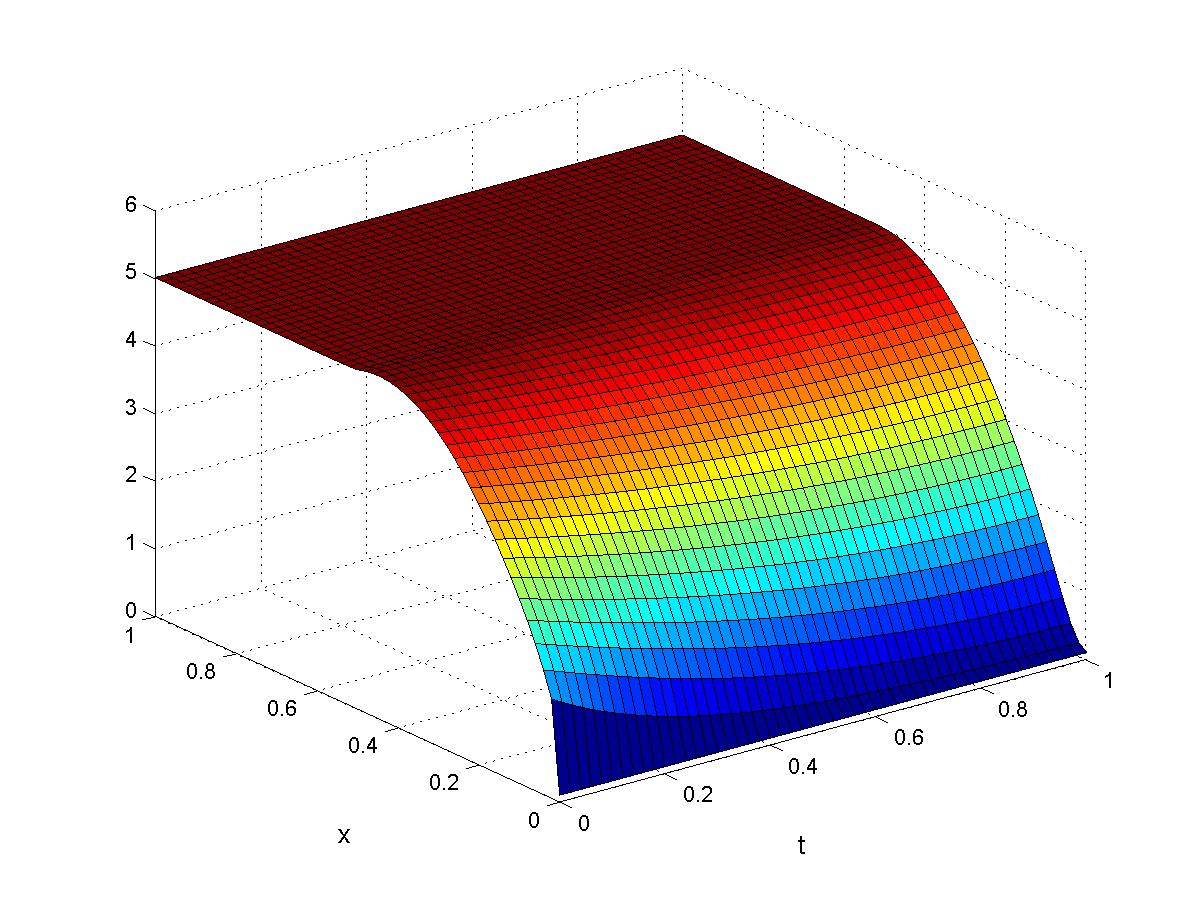
\includegraphics[width = 10cm]{screen.png}
\caption{Распространение тепла в стержне}
\label{fig:1}	
\end{figure}
\end{document}